\documentclass[numbers=noenddot, 12pt, a4paper, oneside]{scrbook}
\usepackage{blindtext}
\usepackage[utf8]{inputenc}
\usepackage{float}
\usepackage{tabularx}
\usepackage{graphicx}
\def\Plus{\texttt{+}}
\usepackage[final]{pdfpages}


\usepackage{listings}
\usepackage{alloy}
\usepackage{xcolor}
\usepackage{color}
\definecolor{alloy-keyword}{rgb}{0.23, 0.23, 0.7}
\definecolor{alloy-comment}{rgb}{0.18, 0.64, 0.18}
\definecolor{alloy-string}{rgb}{0.71, 0.18, 0.71}
\begin{document}
	
\lstset{
	language=alloy,
	numbers=left,
	numberstyle=\tiny,
	stepnumber=2,
	tabsize=4,
	keywordstyle=\color{alloy-keyword}\bfseries,
	commentstyle=\color{alloy-comment},
	stringstyle=\color{alloy-string},
	basicstyle=\small\fontfamily{pcr}\selectfont,
}
 
\begin{titlepage}
	\centering
	{\scshape\LARGE Politecnico di Milano \par}
	\vspace{1cm}
	
\includegraphics[width=0.65\textwidth]{polimi-logo}\par
	\vspace{1cm}
		
	{\scshape\Large Software Engineering 2 Course\par}
	\vspace{1.5cm}
	{\huge\bfseries Travlendar \Plus \par}
	\vspace{6cm}
	{\Large\itshape di\par}
	{\Large\itshape Gianluigi Oliva, Marco Mussi e Lukasz Moskwa\par}
	\vfill

	
	\vfill
	
	% Bottom of the page
	{\large \today\par}
\end{titlepage}

\newpage 
\tableofcontents
\newpage 

\section*{Abstract}

The main task of this document is to give a specification of the requirements that our system has to fulfil adopting the IEEE-STD-830-1993 standard for RASD documentation . It also introduces the functional and non-functional requirements via UML diagrams and a high level specification of the system. In the last part of this document it presents the formal model of the specification using Alloy analysis. \\

The information in this document are intended for the stakeholders and the developers of the project. For the stakeholders this document presents a description useful to understand the project development, meanwhile for the developers it’s an useful way to show the matching between the stakeholders’ requests and the developed solution.

\newpage

\chapter{Introduction}

In this section we will explain which are the main scopes of the Travlendar+ application and we will provide a general overview of all the features.

\section{Purpose}

The main purpose of the RASD document (Requirement Analysis and Specification Document) is to highlight the domain in which the system will work and the primary use cases.\\

The document below specifies who will use the system, the reason for which the system is developed, what services will be provided and the environment in which the system finds its use.
We will need to define the functional and not functional requirements of the system. \\

The main goals to be achieved are:
\begin{itemize}
	\item The user wants to schedule his meetings
	\item The user wants to reach the place of his meeting with the most optimized path
	\item The user wants to know the weather forecast to be better organized for the journey
	\item The user wants to use the means of transport he prefers
	\item The user wants to purchase the tickets for the used means of transport 
	\item The user wants to localize means of shared transport whenever they are around him
	\item The user wants to be sure there are no overlapping in his schedule
	\item The user wants to keep a range of time for his breaks
	\item The user wants to use only a specific kind of means of transport
	\item The user wants to modify his meetings ad rearrange his schedule 
	\item The user wants to share the time of his meetings
\end{itemize}

\section{Scope}

The scope of this application (Travlendar \Plus) is provide a tool for the target users to schedule in an effective way their time optimizing the travels.\\

Travlendar+ allows to create a calendar which fits the meetings and other kind of commitments.
The key feature of this application is to determine if the meeting location is reachable in the scheduled time and then provide a fast way to get to the destionation, otherwise it notify the user that it is not possibile by any mean to fullfill the request. Furthermore the application also arranges the schedule in a flexible way for some kind of events (like the lunch) and offers the possibility to slightly change its time.\\

In the creation of the user's calendar it also takes into account the current weather condition to make smarter decisions. As example, if the user show interest in using bike or a bike sharing service, during a sunny day, the system will favor a suitable path.\\

The user is invited to provide his order of preferences in terms of means of transport. In this way, he is free to choose if use bus, train or subway in a particular day. It is possible to select as well if you want to use a car or bike (your or a sharing service's one). The system also retrieves information about the current path situation like traffic jam or strikes and immediatly find alternative solutions.\\

With Travlendar+ is possible as well to buy public transport's tickets on the fly for the journey. If the user requires often the same path, he is suggested by the application to buy the best offered subscription.


\section{Definitions, Acronyms, Abbreviations}

\subsection*{Definitions}
\begin{itemize}
	\item \textbf{Platform}: system/application as a whole.
	\item \textbf{User}: An end user who is currently registered to the Travlendar+ application and has credentials to access.
	\item \textbf{Guest}: Person not registered yet and with limited access to features.
	\item \textbf{Event}: A scheduled meeting or other kind of appointment a user has to attend.
	\item \textbf{Journey}: The path chosen by the application as the one with all the fullfilled requirements.
	\item \textbf{Bad Weather}: A weather that prevents the user from choosing some path options. The listed bad weathers are snow, rain, storm and others.
	\item \textbf{Framework}: Reusable set of libraries or classes for a software system.
	\item \textbf{Cross-Platform}: software able to run on different platforms with same code.
	\item \textbf{Port}: in the internet protocol suite, it is an endpoint of communication in operating system
\end{itemize}

\subsection*{Acronyms}

\begin{itemize}
	\item \textbf{RASD}: Requirements Analysis and Specification Document
	\item \textbf{DB}: Database
	\item \textbf{DBMS}: Database Management System
	\item \textbf{OS}: Operating System 
	\item \textbf{HTML}: HyperText Markup Language
	\item \textbf{CSS}: Cascading Style Sheets
	\item \textbf{JS}: JavaScript
	\item \textbf{JSON}: JavaScript Object Notation
	\item \textbf{API}: Application Programming Interface
	\item \textbf{IDE}: Integrated Development Environment
	\item \textbf{RAM}: Random Access Memory
	\item \textbf{HTTP}: HyperText Transfer Protocol
	\item \textbf{HTTPS}: HyperText Transfer Protocol Secure
	\item \textbf{TCP}: Transmission Control Protocol
	
\end{itemize}

\subsection*{Abbreviations}
\begin{itemize}
	\item \textbf{Gn}: n-th goal
	\item \textbf{Rn}: n-th functional requirement
	\item \textbf{Dn}: n-th domain
	\item \textbf{Mn}: n-th mockup
	\item \textbf{WebApp}: WebApplication 
\end{itemize}


\section{Revision History}

Version, date and summary\\

\begin{tabular}{|p{0.2\textwidth}|p{0.3\textwidth}|p{0.4\textwidth}|}
	\hline
	\parbox[c][6ex]{6ex}{\centering \textbf{Version}} & \textbf{Date} & \textbf{Summary}\\
	\hline
	\parbox[c][6ex]{6ex}{\centering 1.0.0} & \today & First release of this document\\
%	\parbox[c][6ex]{6ex}{\centering \textbf{Goal}} & 2 \\
	\hline
	
	
	
\end{tabular}


\section{Reference Documents}

We used the following documents:
\begin{enumerate}
	\item The orginal Travlendar application: \\
	\textbf{http://score-contest.org/2018/projects/travlendar.php}
	\item The revised document of the assignment:\\
		\textbf{https://goo.gl/9m1ojy}
	
	\item IEEE Std 830-1998 IEEE Recommended Practice for Software Requirements Specifications. 
	
	\item IEEE Std 1016tm-2009 Standard for Information Tecnology-System Design-Software Design Descriptions.
\end{enumerate}

\section{Document Structure}

This document is composed by the following sections:

\begin{itemize}
	\item \textbf{Section 1:} General overview of the Travlendar+ application and definition of the goals.
	\item \textbf{Section 2:} Overall description of the software feature and implemeted functions. Considerations about constraints, assumptions and dependecies.
	\item \textbf{Section 3:} Specification of functional and not functional requirements in a software and hardware perspective. Examination of design and performance.
	\item \textbf{Section 4:} Formal analysis of requirement using modeling language as Alloy.
	\item \textbf{Section 5:} Time and resource effort during the development of the application.
	\item \textbf{Section 6:} References and software used during the process of creation of the system. 
\end{itemize}


\chapter{Overall Description}

\section{Product Perspective}

We are going to release a cross-platform web application which will be able to run on every device. This application won't provide an interface for the service administrator, because it is possible from the server side.\\

As we are developing a WebApp, we are willing to release custom API for any future application in order to facilitate further implementations.\\

\subsection*{World and Machine model interpretation}

\begin{figure}[H]
	\centering
	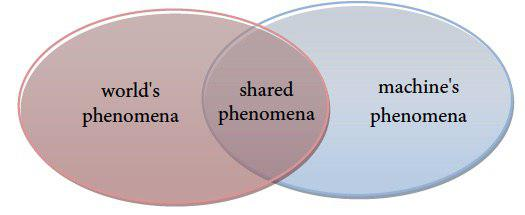
\includegraphics[width=0.8\textwidth]{phenomena}
	\caption{Relation between world and machine phenomena}
\end{figure}

From now on we will refer to \textbf{world} as everything that not concern our system and \textbf{machine} as everything about our system. Therefore \textbf{world's phenomena} are all the external events happening in the world and \textbf{machine's phenomena} are the events related to the system. There are as well some \textbf{shared phenomena} which are observable by both the parts.\\

In our case the world's phenomena are:
\begin{itemize}
	\item Bus out of service or other mechanical failure in public transports
	\item Closed roads due to a public demonstration
\end{itemize}
In our case the machine's phenomena are:
\begin{itemize}
	\item Estimation and managing of users' free time 
	\item Database query
	\item User's registration
\end{itemize}
In our case the shared phenomena are:
\begin{itemize}
	\item Tracking of public transport's means
	\item Strikes and public services manifestation
\end{itemize}


\section{Product Functions}

The product provide to users a simple and user-friendly interface to schedule their events and help them to organize their journey.\\

In particular the system is expected to be able to:
\begin{itemize}
	\item Let the guest register and log in as users
	\item Schedule several events for every user
	\item Computate the best possible path for the daily journey
	\item Notify the user if the current journey is not realizable and why
	\item Interact with third part and sharing services 
	\item Let the user buy tickets for the ride
	\item Support the user during the whole travel
	\item Allow the user to insert his preferred choice for the used transports
	\item Gives a real time evaluation of the environmental conditions (like strikes and weather situation) and uses it to find the best choice for the journey.
\end{itemize}

\section{User Characteristics}


We don't require the user to be particulary skilled in new technologies as we expect the users to be aware and capable of using basic functions of mobile devices.\\

The actors we identified are:
\begin{itemize}
	\item \textbf{Guests}: people that haven't yet gained credentials to access the full service are only able to check the best journey options with some restrictions: they cannot save their schedule nor buy tickets or use third part sharing services.
	\item \textbf{Users}: guests that are currently registered to Travlendar+ and already verified their credentials (as e-mail address). Such users are able to log in and access full service with no restrictions.
\end{itemize}
\section{Assumptions, Dependencies and Constraints\\}

\subsection*{Costraints}

\begin{itemize}
	\item \textbf{Hardware limitations}: Our application runs on every mobile device like smartphones and tablets, independently of the OS (will run on Android, iOS and Windows Phone). Therefore, as the App consumes a low amount of RAM, the only hardware constraint for the users is to have a mid-range device. (for instance Nexus 4 or better for Android, iPhone 5 or better for iOS and Nokia Lumia 520 for Windows Mobile).
	\item \textbf{Interface to other applications}: The system needs to interfaces itself with other third part applications in order to provide the capability of buying tickets and booking sharing services.
	\item \textbf{Parallel operations}: The application must be able to handle multiple parallel requests from several users granting a high reactivity.
	\item \textbf{Availability limitations}: The system's uptime and availability are around the 98\% corresponding to a maximum downtime of $3.36h$ per week.
	\item \textbf{Privacy Constraints}: The personal informations of the users, as for instance the current geo-position, must be safely stored and not reachable to other people.
\end{itemize}


\subsection*{Assumptions and Dependecies}
\begin{itemize}
	\item \textbf{Internet Connection}: the device used by the users dispose of an internet connection and a sufficient bandwidth to use the application.
	\item \textbf{Device GPS}: the device used by the users dispose of a built in GPS Localizer.
	\item \textbf{Public transports tracking}: all the public transports are real time localized
	\item \textbf{No privileged users}: there are no priviled users or administrators with particular functions
	\item \textbf{No user connections}: every user is independent from the others, and their schedule does not affect by any mean the others schedules
	\item \textbf{Weather information not available}: when the weather informations are not available, the system computates the schedules without considering them
	\item \textbf{Booking range}: we assume that the users are not interested in planning events that will occur later than a week
	\item \textbf{City Location}: the users live and uses the application in the surroundings of Milan
	\item \textbf{Weather information provided}: we assume that the weather informations are correct and provided by a third part
	\item \textbf{Shared services provided}: we assume that the sharing services are working and provided by a third part
	\item \textbf{Host availability}: the server which hosts the application has an uptime greater or equal to the uptime of the application
	\item \textbf{Battery duration}: user's device's battery duration is enough to permit the fullfillment of the journey.
	\item \textbf{API availability}: the API provided by third part's services are always available
	\item \textbf{Break/Lunch time}: we assume that the user will eat near the same place of the event before the break.
	\item \textbf{OS Permission Granted}: the user will always grant to his OS's device the permission to access to all the needed services
\end{itemize}

\chapter{Specific Requirements}

\section{External Interfaces Requirements}
\subsection*{User Interface}

The user interface must be user-friendly volted to guarantee to the final user an easy way to interact with the application. The development of the front end is realized due to HTML and CSS to provide a responsive interface for all devices.\\

\begin{figure}[H]
	\centering
	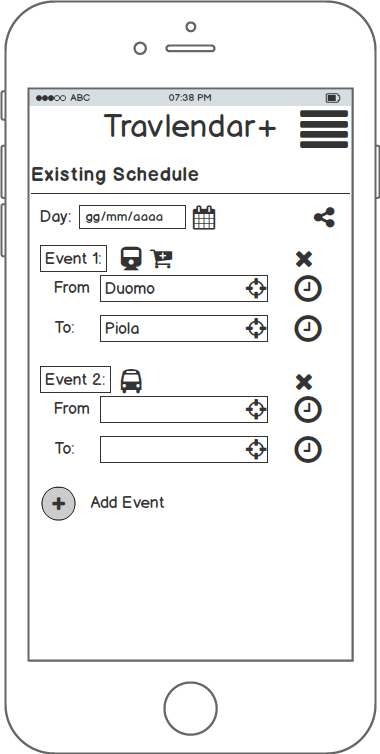
\includegraphics[width=0.7\textwidth]{mockups/ExistingSchedule}
	\caption{Mockup: In this interface the user can see his already created schedules and events }
\end{figure}

\begin{figure}[H]
	\centering
	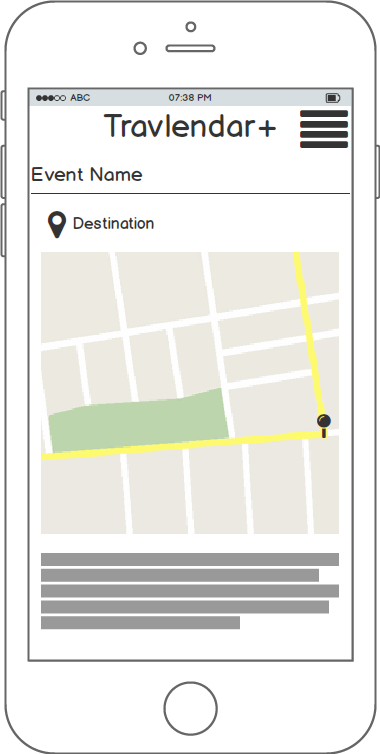
\includegraphics[width=0.7\textwidth]{mockups/Guide}
	\caption{Mockup: This interface shows up to the user of the preview of his journey to reach the selected event}
\end{figure}

\begin{figure}[H]
	\centering
	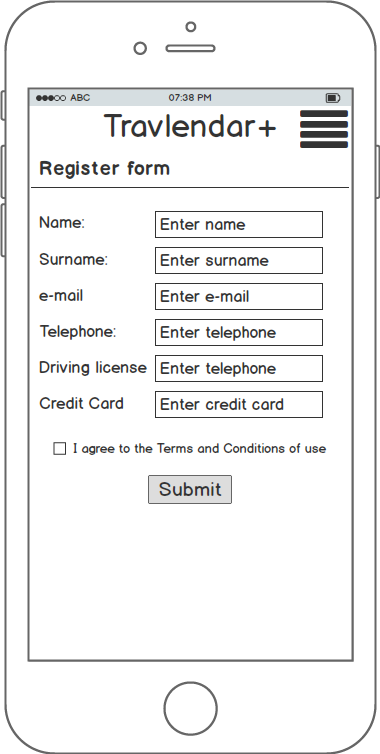
\includegraphics[width=0.7\textwidth]{mockups/Login}
	\caption{Mockup: This interface allow the user to perform the login action}
\end{figure}

\begin{figure}[H]
	\centering
	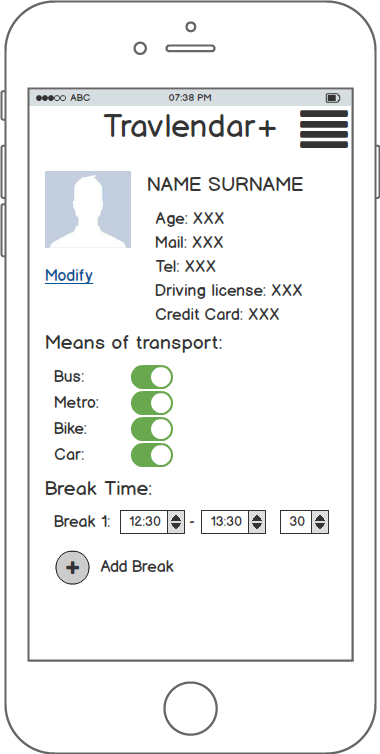
\includegraphics[width=0.7\textwidth]{mockups/PersonalArea}
	\caption{Mockup: In this section the user is able to view and modify his personal data}
\end{figure}

\begin{figure}[H]
	\centering
	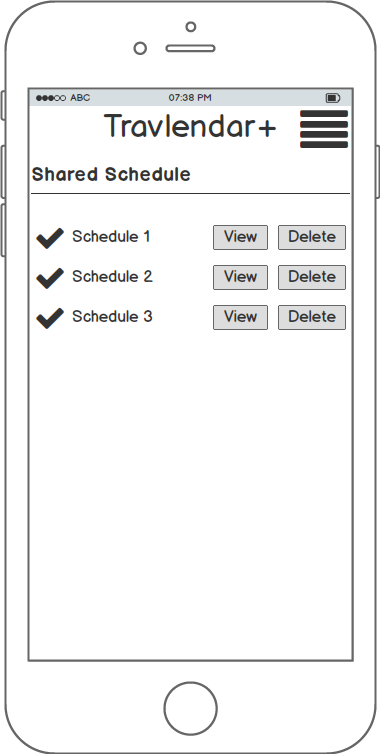
\includegraphics[width=0.7\textwidth]{mockups/SharedSchedule}
	\caption{Mockup: This interface shows to the user the schedules that are actually shared with him}
\end{figure}

\begin{figure}[H]
	\centering
	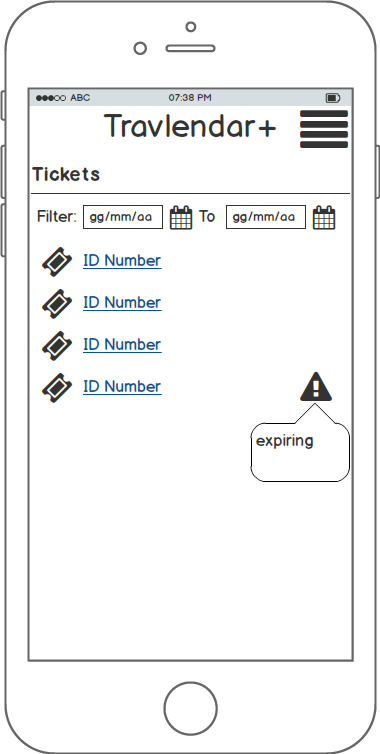
\includegraphics[width=0.7\textwidth]{mockups/Tickets}
	\caption{Mockup: In this section the user can see the tickets and subscriptions history}
\end{figure}

\begin{figure}[H]
	\centering
	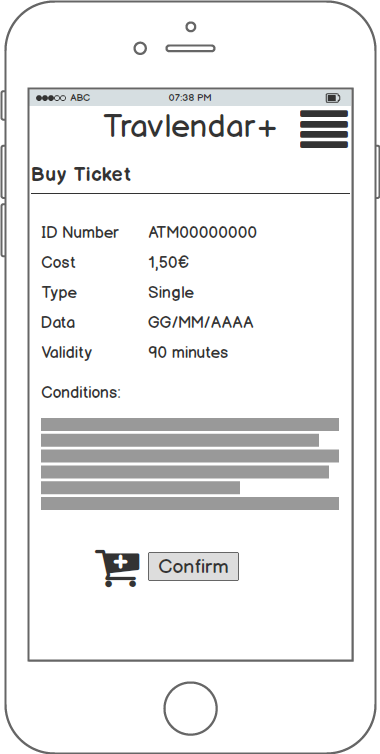
\includegraphics[width=0.7\textwidth]{mockups/TicketsBuy}
	\caption{Mockup: This interface allow the user to perform the buy operation and complete his transaction}
\end{figure}

\subsection*{Hardware Interface}

The system must be able to acquire the correct position of the means of transport and sharing services' vehicles. In order to acquire such data, every mean of transport must have a GPS localizer and internet connection to communicate its position to their server.

\subsection*{Software Interface}

The system in order to be developed, both on the front-end side and back-end side, needs the use of the following programming, markup and representation languages:
\begin{itemize}
	\item JavaScript
	\item HTML
	\item CSS
	\item Python
	\item SQL
	\item JSON
\end{itemize}
There are no particular limitation about the OS of the user's devices, as the application is cross-platform and can be also used with modern browsers.

\subsection*{Communication Interface}

The communication between client and server happens using HTTPS by TCP protocol using port 443. A crypted channel is also used in order to perform secure transactions with third part sellers.

On the other hand the connection which allow to download public informations from third part API provided by major services like Google uses HTTP with port 80.

\section{Functional Requirements}
The user must be able to:
\begin{enumerate}
	\item Register to Travlendar+ application.\\ The system:
	\begin{itemize}
		\item Provides a form to insert all the personal information like name, surname, e-mail...
		\item Verifies the genuineness of the e-mail address by sending an e-mail with a confirm request
	\end{itemize}
	\item  Create a daily schedule specifying the location in which the event will take place and its timetable.\\
	The system:
	\begin{itemize}
		\item Provides a form to be fullfilled with all the information about the event
		\item Checks that all the relevant fields were compiled in order to approve the request
		\item Provides a method to prove that the request was confirmed
		\item Deletes all unsaved changes to the planning if the internet connection is absent or the application server is down
		\item Finds the best route solution starting from some user's parameters
		\item Notifies the user whenever the given parameters lead to an impossible solution
		\item Takes in account the weather condition when looking for the best mean of transport and provides the options that can be selected by the user
		\item Track the user initial position throught the GPS or an inserted address
		\item Notifies the user if there is a lack of internet connection and therefore a restriction to the application's services
	\end{itemize}
	\item Manage his own data.\\The system:
	\begin{itemize}
		\item Provides a method to change all the user's data like e-mail, telephone number..
		\item Requires another e-mail verification in case the original e-mail was changed
		\item Let the user modify his preferences about the desired means of transport
		\item Let the user set or modify his preferences about the desired break time interval and how much it lasts
	\end{itemize}
	\item Retrieve informations about the weather forecast in a specified range of dates
	\\The system:
	\begin{itemize}
		\item Allows the user to select the date to check the weather in
		\item Retrieves the datas about the weather forecast
		\item Uses the GPS position in order to retrieve the informations about the city the user is requesting the forecast for
	\end{itemize}
	\item Buy tickets and subscription for public transports.\\The system:
	\begin{itemize}
		\item Provides the user all possible choices to perform a payment (like PayPal, Credit Card and other kinds of money transfer)
		\item Notifies the user, whenever a fail occurs, the reason why it failed
		\item Runs along with third parts applications to fullfill the request
		\item Memorizes all the bought or already owned tickets or subscriptions
		\item Provides an easy and accessible way to visualize already bought tickets
		\item Notifies the user if any of the subscription are evaluated
	\end{itemize}
	\item Share his own daily schedule with other users.\\The system:
	\begin{itemize}
		\item Provides an easy way to share datas with other users
		\item Saves the received shared schedule to be seen later
	\end{itemize}
	\item Modify an already compiled schedule for a certain day.\\The system:
	\begin{itemize}
		\item Provides a method to allow the user to reschedule the timetable with new preferences
		\item Notifies the user whenever his changes lead to a non optimal or impossibile solution 
		\item Let the user delete an already created schedule
	\end{itemize}
	\item Choose his preferred time for having a meal.\\The system:
	\begin{itemize}
		\item Let the user decide the range of time when he wants to eat and the preferred time
	\end{itemize}
	\item Receive information about the current journey.\\The system:
	\begin{itemize}
		\item Provides all the informations about the selected journey showing the way to travel
		\item Shows any information about the current traffic jam and road works
		\item Informs the user about the waiting time for public transports
	\end{itemize}
\end{enumerate}
\newpage
\section*{Scenario, Use case diagrams and Flow Diagram}


\subsection*{Scenario 1}

Mark has already bought a new smartphone so he decide to change the application to manage his timetable with the scope to optimize his schedule. So he decides to sign up Travlendar+ Application from his smartphone.
First of all he downloads the application from the smartphone’s store and, once is installed on the device, he fills all the field the registration form in the correct way and, once he confirms the authenticity of the e-mail address, he can join all services provided by the application.\\
\begin{figure}[H]
	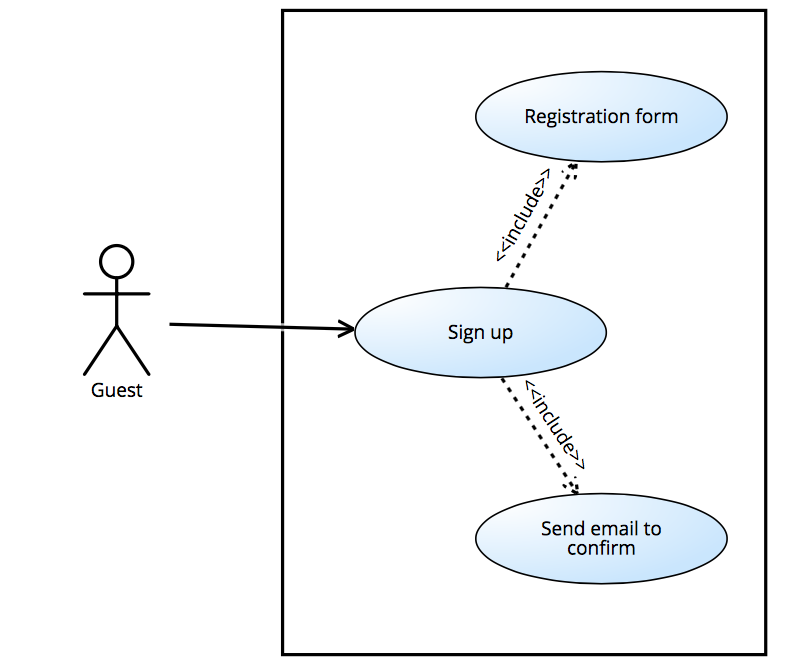
\includegraphics[width=1\textwidth]{usecases/Scenario1}
	\caption{Use Case: Sign up}
\end{figure}


\begin{tabular}{|c|p{0.8\textwidth}|}
	\hline
	\parbox[c][6ex]{6ex}{\centering \textbf{Name}} & Sign up\\
	\hline
	\parbox[c][6ex]{6ex}{\centering \textbf{Actor}} & Guest \\
	\hline
	\parbox[c][10ex]{15ex}{\centering \textbf{Entry Condition}} & The actor hasn’t got an account on the system\\
	\hline
	\parbox[c][10ex]{12ex}{\centering \textbf{Event Flow}} & \begin{itemize}
		\item The guest download the application and open the application
		\item The guest clicks on sign up button
		\item The application provides the registration form
		\item The guest inserts mandatory data in the form like name, surname,e-mail.
		\item The guest optionally he could provides optional data like phone, driving licence number and the credit card to eventually pay the services linked to the app
		\item The guest agrees about terms and conditions of the service by put a tick in the checkbox
		\item The guest clicks submit button
		\item The system sends entered data to the server
		\item The system sends to his e-mail address a mail with a link to check the e-mail address
		\item The user clicks on the provided address
		\item The system validates the email address and the account
	\end{itemize}\\
	\hline
	\parbox[c][7ex]{12ex}{\centering \textbf{Exit condition}} & The actor become a user of the system and he can use the application. \\\hline
	\parbox[c][10ex]{13ex}{\centering \textbf{Exceptions}} & Some mandatory field are not correctly filled and the system ask to the guest to correct it or the mail is not correct so is not possible to complete the sign up and the guest must redo the operation filling the field corresponding with the correct e-mail address.
	Also if he don’t agree with terms and condition of the service, the application provide an error message and ask to check the corresponding box to complete the operation.\\ \\ \hline	
	
	
\end{tabular}

\begin{figure}[H]
	\centering
	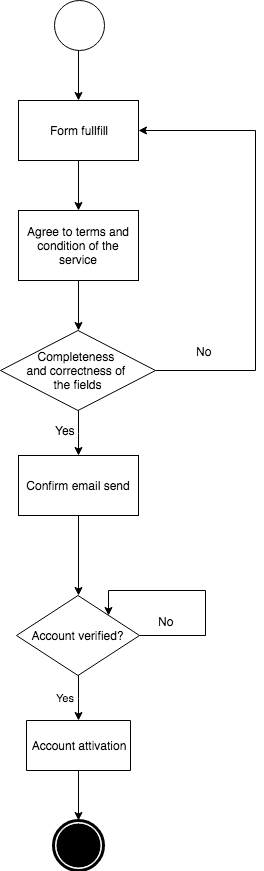
\includegraphics[width=0.4\textwidth]{flows/Scenario1}
	\caption{Activity Diagram: Sign up}
\end{figure}

\newpage
\subsection*{Scenario 2}

Susan performs the login from her own mobile device because she wants to schedule a work's meeting that she will attend near Cairoli. Immediately after she has to move near Navigli to attend hers friend birthday party. In order to do so she access to the event creation's dedicated section completing the proposed form with all the requested informations about the meeting (like the time it starts and ends). Then, the system calculates every possible journey solution based on the user's previously inserted preferences and the weather conditions. After she completes the creation's procedure selecting the best means of transport, Susan insert as well the informations about the birthday party and performs the same operations.
\\

\begin{figure}[H]
	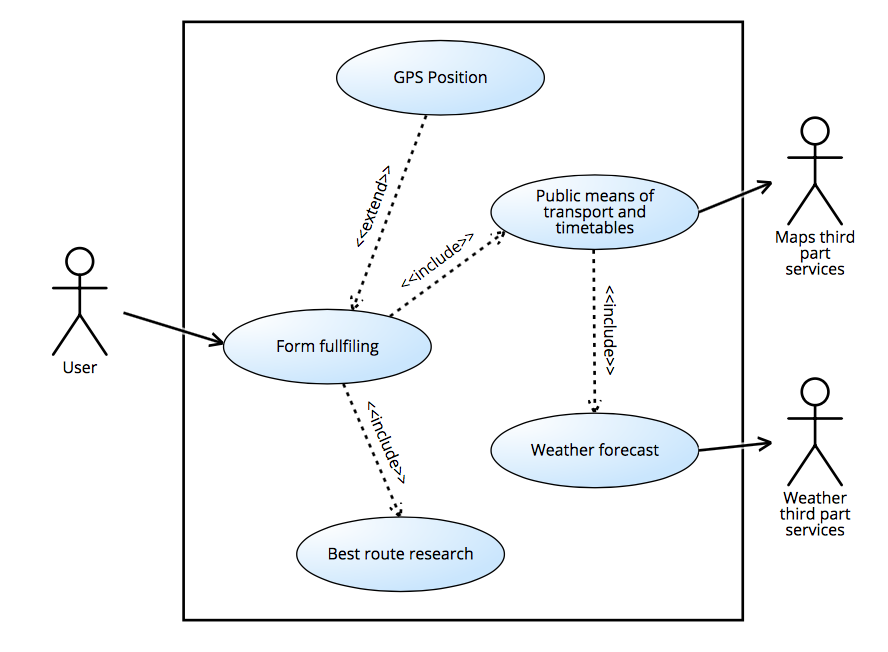
\includegraphics[width=1\textwidth]{usecases/Scenario2}
	\caption{Use Case: Schedule creation}
\end{figure}

\begin{tabular}{|c|p{0.8\textwidth}|}
	\hline
	\parbox[c][6ex]{6ex}{\centering \textbf{Name}} & Schedule creation
	\\
	\hline
	\parbox[c][6ex]{6ex}{\centering \textbf{Actor}} & User, Weather third part services, Maps third part services \\
	\hline
	\parbox[c][10ex]{15ex}{\centering \textbf{Entry Condition}} & The user is already logged in with his username and password
	\\
	\hline
	\parbox[c][10ex]{12ex}{\centering \textbf{Event Flow}} & \begin{itemize}
		\item The user select the "Schedule creation" section from the lateral menu
		\item The user fullfill the form selecting the event date, time and the starting location (using an address or clicking the icon for using GPS position) and the destination location
		\item The user press the confirm button
		\item The system request the information about all the possible routes to calculate to Maps third part services
		\item The system calculates the best route based on the user's previously selected preferences
		\item The system shows to the user the proposed solution
		\item The user confirms the schedule
		\item The system stores in the database the selected schedule for the user
		
		
	\end{itemize}\\
	\hline
	\parbox[c][7ex]{12ex}{\centering \textbf{Exit condition}} & The user creates a schedule that supports him in reaching on time his destinations \\\hline
	\parbox[c][10ex]{13ex}{\centering \textbf{Exceptions}} & Some exception can occur: if the user doesn't fill all the form's fields the system notifies it and ask the user to compile them again. If the destinations location is not reachable in the given time or there isn't any possible route traceable the system notifies the user and delete the current operation. The user refuses the created schedule and the system deletes the current operation. If the internet connection is dropped while the operation is ongoing the system deletes the operation and notifies the user.
	
	\\\hline	
	
	
\end{tabular}

\begin{figure}[H]
	\centering
	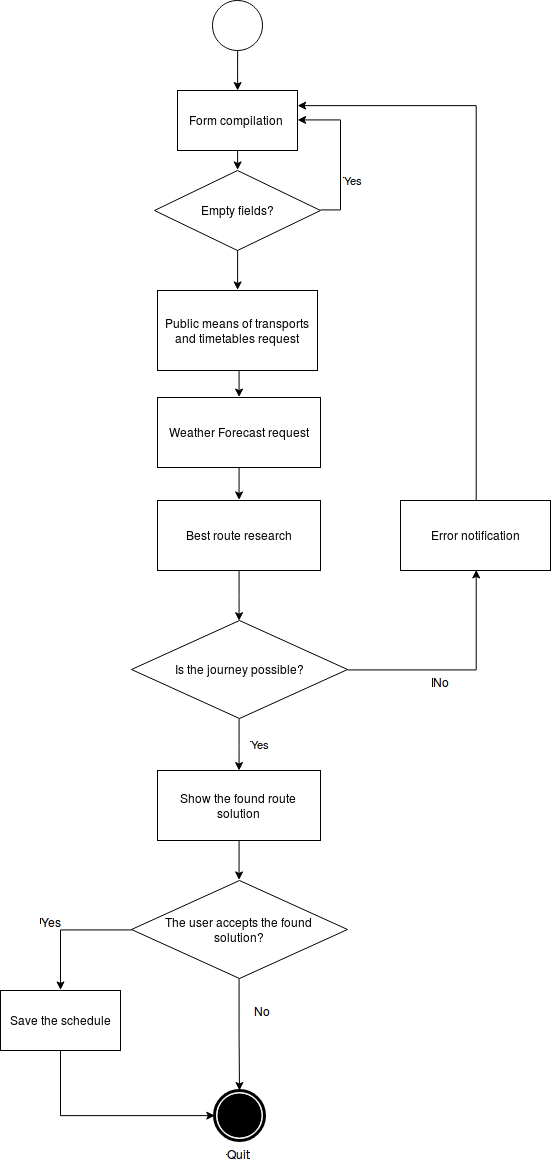
\includegraphics[width=0.65\textwidth]{flows/Scenario2}
	\caption{Activity Diagram: Schedule creation}
\end{figure}

\subsection*{Scenario 3}

Mark hear from her friend Susan that the application could be personalized with the purpose to better adapt to the user needs so he decides to look at the user’s informations page and modify his profile to adapt it.
He hate to use the bus because he thinks it is too slow and require a lot of time to reach the destination using so he switch off the corresponding field.\\


\begin{figure}[H]
	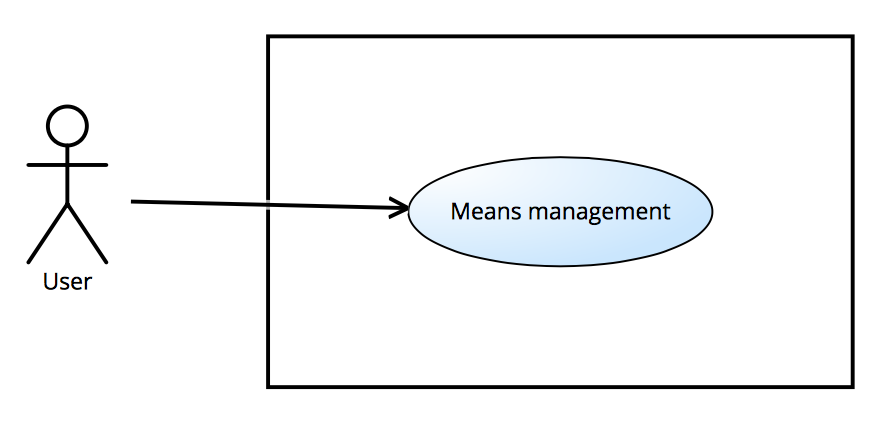
\includegraphics[width=1\textwidth]{usecases/Scenario3}
	\caption{Use Case: Manage his preference about means of transport}
\end{figure}

\begin{tabular}{|c|p{0.8\textwidth}|}
	\hline
	\parbox[c][6ex]{6ex}{\centering \textbf{Name}} & Manage his preference about means of transport
	\\
	\hline
	\parbox[c][6ex]{6ex}{\centering \textbf{Actor}} & User \\
	\hline
	\parbox[c][10ex]{15ex}{\centering \textbf{Entry Condition}} & The user already logged want to select his preferences about means of transport
	\\
	\hline
	\parbox[c][10ex]{12ex}{\centering \textbf{Event Flow}} & \begin{itemize}
		\item The user clicks on the menu button and find the page about the account management
		\item The system provides all the information that it know about the user and permit to modify all data defined editable.
		\item The user find the switch corresponding to the bus option and turn off it
		\item The system update the user preferences
		
	\end{itemize}\\
	\hline
	\parbox[c][7ex]{12ex}{\centering \textbf{Exit condition}} & User setted the preferences about the bus \\\hline
	\parbox[c][10ex]{13ex}{\centering \textbf{Exceptions}} & The user turn off all the switch so the application return an error message 
	\\ \\ \hline	
	
	
\end{tabular}
\begin{figure}[H]
	\centering
	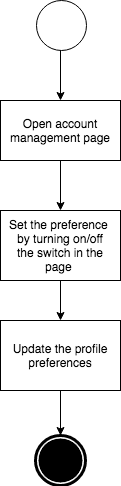
\includegraphics[width=0.3\textwidth]{flows/Scenario3}
	\caption{Activity Diagram: Manage his preference about means of transport}
\end{figure}
\newpage

\subsection*{Scenario 4}

Susan performs the login operation from her own mobile device because she wants to check the Monday's weather conditions and know how to dress for her city festival. In order to do so she access the "Weather Forecast" section from the lateral menu and insert the date she is interested in. The system the requests Weather third part services' informations and shows the weather conditions.
\\

\begin{figure}[H]
	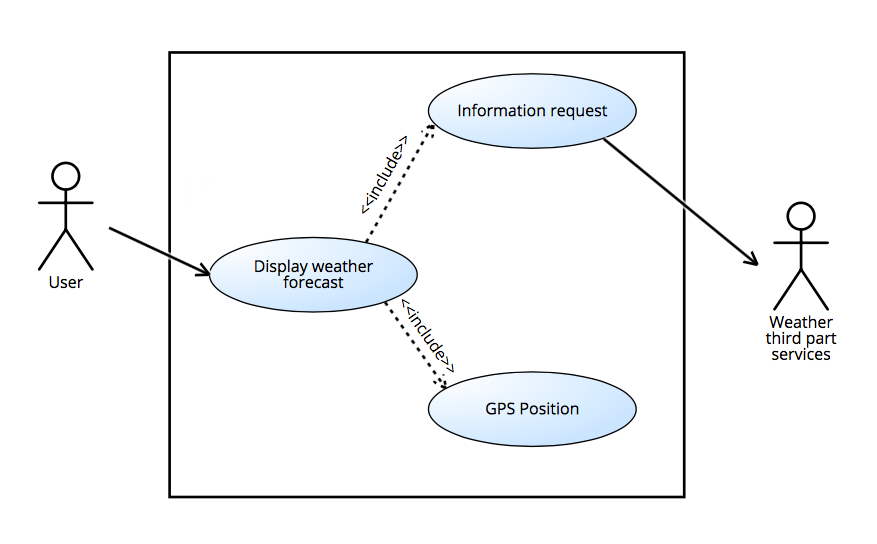
\includegraphics[width=1\textwidth]{usecases/Scenario4}
	\caption{Use Case: Weather Forecast consulting}
\end{figure}

\begin{tabular}{|c|p{0.8\textwidth}|}
	\hline
	\parbox[c][6ex]{6ex}{\centering \textbf{Name}} & Weather Forecast consulting
	
	\\
	\hline
	\parbox[c][6ex]{6ex}{\centering \textbf{Actor}} & User, Weather third part services
	 \\
	\hline
	\parbox[c][10ex]{15ex}{\centering \textbf{Entry Condition}} & The user already logged want to select his preferences about means of transport
	\\
	\hline
	\parbox[c][10ex]{12ex}{\centering \textbf{Event Flow}} & \begin{itemize}
		\item The user selects the "Weather Forecast" section from thee lateral menu
		\item The user inserts the date of the day he is interested retrieving information in
		\item The system uses the GPS to determine the current user's current position
		\item The system interacts with Weather third part services to request the information about the weather forecast
		\item The system shows to the user the information received
		
		
	\end{itemize}\\
	\hline
	\parbox[c][7ex]{12ex}{\centering \textbf{Exit condition}} & The user obtains the informations about the forecast required\\\hline
	\parbox[c][10ex]{13ex}{\centering \textbf{Exceptions}} & Some exceptions can occur if: the user inserts a date which is over a certain range. If the GPS position is not available the system notifies the user with an error message. If the weather forecast information are not available the system notifies the user.
	 
	\\ \\ \hline	
	
	
\end{tabular}

\begin{figure}[H]
	\centering
	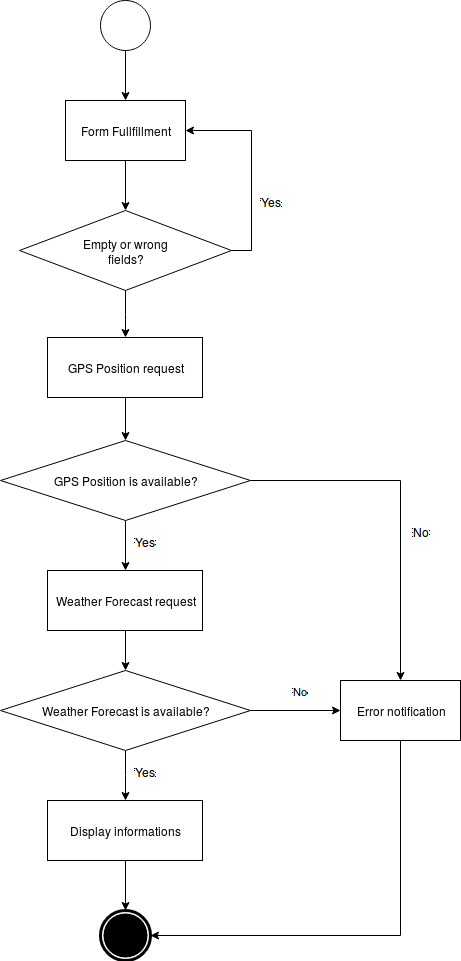
\includegraphics[width=0.65\textwidth]{flows/Scenario4}
	\caption{Activity Diagram: Weather Forecast consulting}
\end{figure}

\subsection*{Scenario 5}

John is a common Travlendar+ user and very often needs the application in order to schedule his appointments during the day. Sometimes he is so busy that he actually forgets to renew his weekly bus subscription. John isn't worried about that, because he knows that he can do it manually using Travlendar+ which will automatically allow him to choose his preferred payment method and perform the transaction when he creates the event. After the transaction, John wants to be sure that the ticket is actually there, so he checks his Tickets section, where all his tickets are stored.
\\

\begin{figure}[H]
	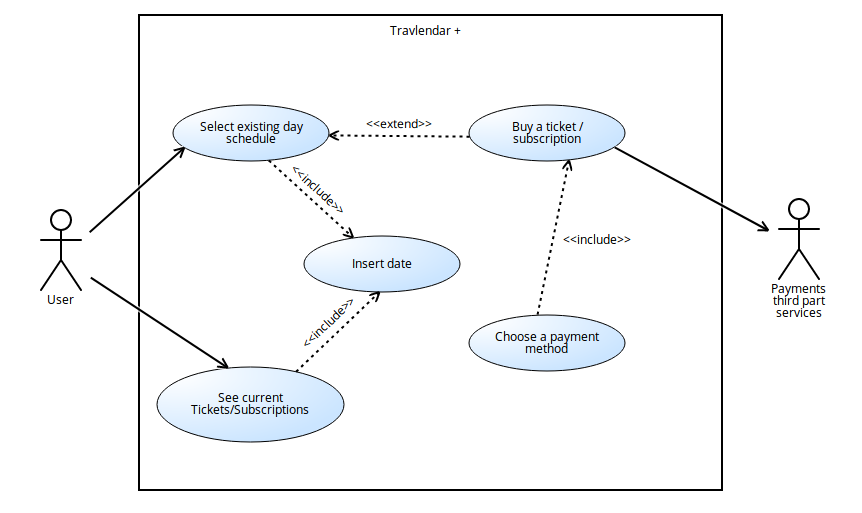
\includegraphics[width=1\textwidth]{usecases/Scenario5}
	\caption{Use Case: Buy tickets and subscription for public transport}
\end{figure}

\begin{tabular}{|c|p{0.8\textwidth}|}
	\hline
	\parbox[c][6ex]{6ex}{\centering \textbf{Name}} & Buy tickets and subscription for public transport
	\\
	\hline
	\parbox[c][6ex]{6ex}{\centering \textbf{Actor}} & User, Google third part services, Payments third part services
	\\
	\hline
	\parbox[c][10ex]{15ex}{\centering \textbf{Entry Condition}} & The user already logged has to renew on the fly his subscription or buy an occasional ticket
	\\
	\hline
	\parbox[c][10ex]{12ex}{\centering \textbf{Event Flow}} & \begin{itemize}
		\item The user selects from the lateral menu the Existing Schedule section
		\item The user selects the date of the schedule he wants to buy tickets/subscriptions for
		\item The user tap the cart icon if he wants to perform a purchase
		\item The user choose a payment method
		\item The system requires a form for fullfilling the payment transaction
		\item The user complete the form requested
		\item The user press the confirm button
		\item The system interact with the payments third part service to \item complete the transaction
		\item The system store the receipt on the database
		\item The system notifies the user that everything went well
		\item The user selects from the lateral menu the Tickets section
		\item The system shows all the history of payments/tickets
				
	\end{itemize}\\
	\hline
	\parbox[c][7ex]{12ex}{\centering \textbf{Exit condition}} & The user perform the transaction and get the subscription/ticket
	\\\hline
	\parbox[c][10ex]{13ex}{\centering \textbf{Exceptions}} & The user compiles in a wrong way the given form. The ticket selected is not purchasable anymore. There are errors in the payments third part services
	
	\\ \\ \hline	
	
	
\end{tabular}

\begin{figure}[H]
	\centering
	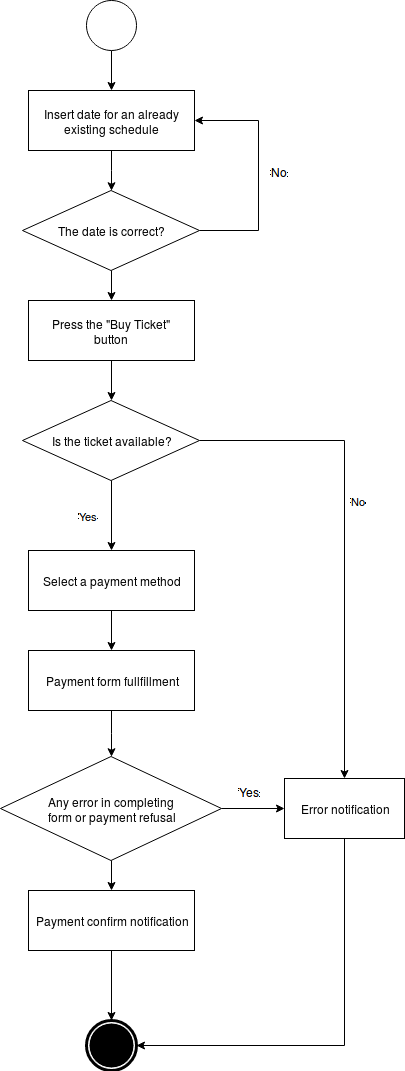
\includegraphics[width=0.5\textwidth]{flows/Scenario5}
	\caption{Activity Diagram: Buy tickets and subscription for public transport}
\end{figure}

\subsection*{Scenario 6}

John is a really busy man, and sometimes he has even like 5 events during the day. Whenever a colleague of his, which is a Travlendar+ user as well, asks him "What are you doing tomorrow?" he doesn't really remember. But John knows that with Travlendar+ it is actually easy to share his daily schedule with other users, so he decide just to send them all his events of a given day.
\\

\begin{figure}[H]
	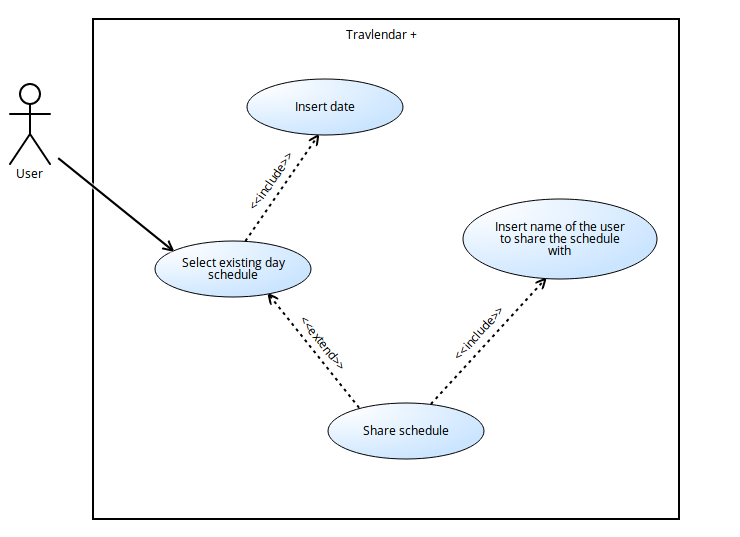
\includegraphics[width=1\textwidth]{usecases/Scenario6}
	\caption{Use Case: Share user's his daily schedule with other users}
\end{figure}

\begin{tabular}{|c|p{0.8\textwidth}|}
	\hline
	\parbox[c][6ex]{6ex}{\centering \textbf{Name}} & Share user's his daily schedule with other users
	\\
	\hline
	\parbox[c][6ex]{6ex}{\centering \textbf{Actor}} & User
	\\
	\hline
	\parbox[c][10ex]{15ex}{\centering \textbf{Entry Condition}} & A user already logged wants to share his daily schedule with another user
	\\
	\hline
	\parbox[c][10ex]{12ex}{\centering \textbf{Event Flow}} & \begin{itemize}
		\item The user selects from the lateral menu the Existing Schedule section
		\item The user selects the date of the schedule he wants to share
		\item The user select the share icon
		\item The user writes the username of another existing user on Travlendar+
		\item The system searches the user associated with the inserted username
		\item The user confirms that he wants to share his daily schedule
		\item The system loads the schedule into the database’s table associated to the other user
		\item The system notifies that the operation has concluded with success
	\end{itemize}\\
	\hline
	\parbox[c][7ex]{12ex}{\centering \textbf{Exit condition}} & The user shares his daily schedule of a given day with another user
	\\\hline
	\parbox[c][10ex]{13ex}{\centering \textbf{Exceptions}} &  The user insert the wrong name of another username, which notifies that the user doesn’t exist. The user inserts a date where there are no schedule already saved. If the internet connection drops while the user is performing such operation or the system is not reachable, the operation gets deleted.
	\\ \\ \hline	
	
	
\end{tabular}

\begin{figure}[H]
	\centering
	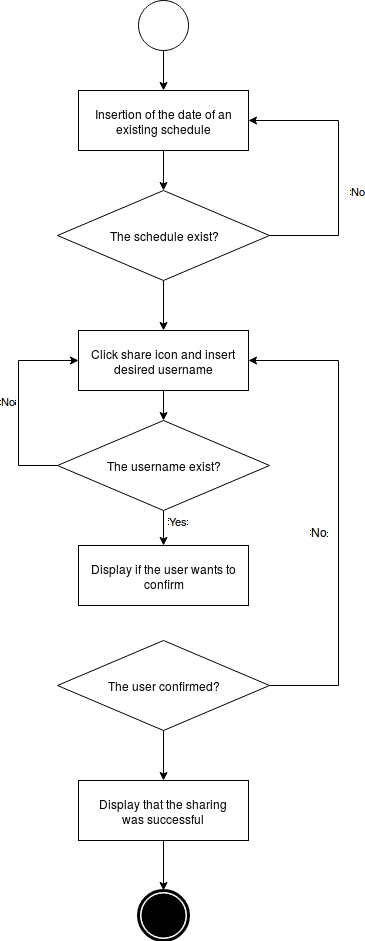
\includegraphics[width=0.5\textwidth]{flows/Scenario6}
	\caption{Activity Diagram: Share user's his daily schedule with other users}
\end{figure}
\newpage

\subsection*{Scenario 7}

Mark wants to reschedule che appointment of the 3pm putting it forward of an hour and wants to know if is possible to reach the destination on time and also if it grants his lunch. He already scheduled the appointment on Travlendar+ o he is looking for moving it an hour before.
So he opens Travlendar+ calendar application, select the event and move.
He sees by the application that is possible and confirm to Anne the moving of the meeting.
\\

\begin{figure}[H]
	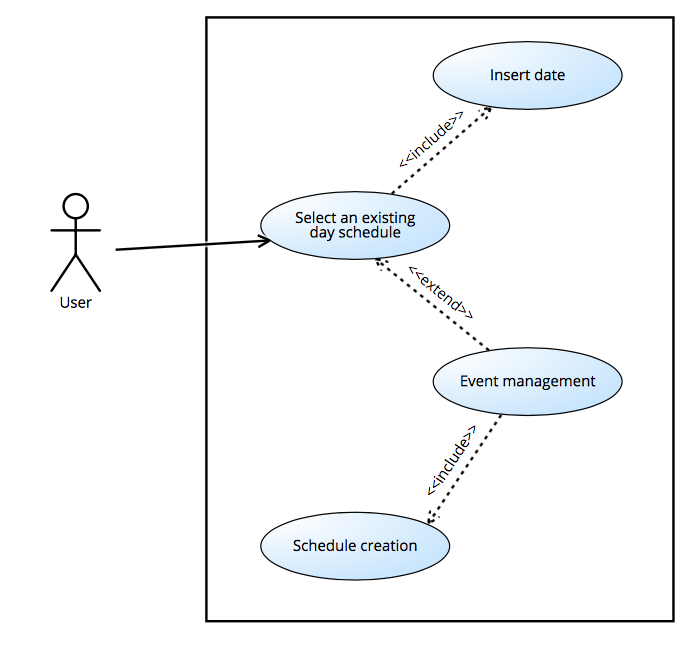
\includegraphics[width=1\textwidth]{usecases/Scenario7}
	\caption{Use Case: Modify an already compiled schedule for a certain day.}
\end{figure}

\begin{tabular}{|c|p{0.8\textwidth}|}
	\hline
	\parbox[c][6ex]{6ex}{\centering \textbf{Name}} & Modify an already compiled schedule for a certain day.
	\\
	\hline
	\parbox[c][6ex]{6ex}{\centering \textbf{Actor}} & User \\
	\hline
	\parbox[c][10ex]{15ex}{\centering \textbf{Entry Condition}} & The user is already logged in and he has already fill his timetable with al least one appointment
	\\
	\hline
	\parbox[c][10ex]{12ex}{\centering \textbf{Event Flow}} & \begin{itemize}
		\item The user selects from the lateral menu the Existing Schedule section
		\item The user insert the data of the event he wants to modify
		\item The system shows all the events of the day
		\item The user clicks on the event he wants to move
		\item The user inserts the updated information
		\item The user confirms the choice
		\item The system calculates the new journey
		\item The system returns a positive feedback so the event updated
	\end{itemize}\\
	\hline
	\parbox[c][7ex]{12ex}{\centering \textbf{Exit condition}} & The user succeed in updating his schedule \\\hline
	\parbox[c][10ex]{13ex}{\centering \textbf{Exceptions}} & The application report an error if the schedule is not feasible. If the user inserts wrong data the system notifies the error. If the selected data does not contains an event the user is notified of the error.
	\\ \\ \hline	
	
	
\end{tabular}

\begin{figure}[H]
	\centering
	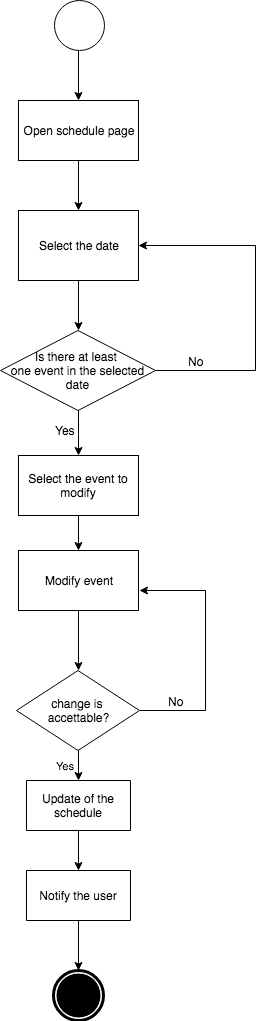
\includegraphics[width=0.35\textwidth]{flows/Scenario7}
	\caption{Activity Diagram : Modify an already compiled schedule for a certain day.}
\end{figure}

\newpage
\subsection*{Scenario 8}

Mark is setting up his own preferences about the means of transport so once here he realize that is possible to set a custom time for the lunch interval and the length that he prefers for the break. He decides that for the lunch is enough thirty minutes and set the time in which he wants to have break.
\\
\begin{figure}[H]
	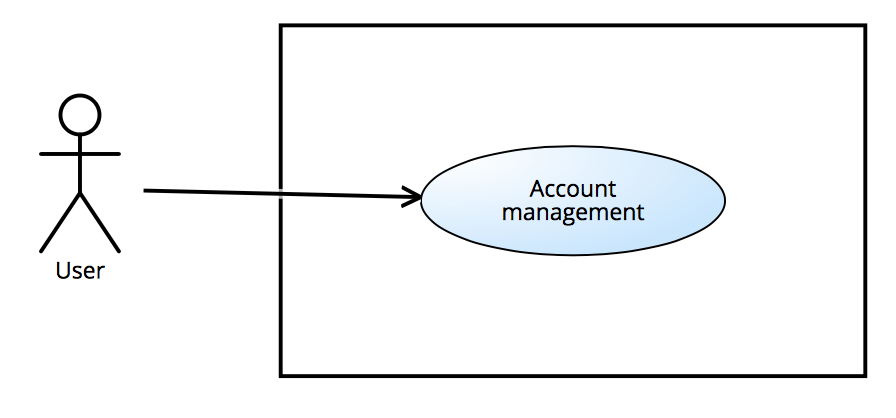
\includegraphics[width=0.7\textwidth]{usecases/Scenario8}
	\caption{Use Case: Manage his preference about time for break}
\end{figure}


\begin{tabular}{|c|p{0.8\textwidth}|}
	\hline
	\parbox[c][6ex]{6ex}{\centering \textbf{Name}} & Manage his preference about time for break
	\\
	\hline
	\parbox[c][6ex]{6ex}{\centering \textbf{Actor}} & User \\
	\hline
	\parbox[c][10ex]{15ex}{\centering \textbf{Entry Condition}} & The user is already logged in and wants to change his preferences
	\\
	\hline
	\parbox[c][10ex]{12ex}{\centering \textbf{Event Flow}} & \begin{itemize}
		\item The user clicks on the menu button and find the page about the account management
		\item The system provides all the information that it know about the user and permit to modify all data defined editable
		\item The user inserts the desired hour that he is used to have break
		\item The user inserts the estimate duration of the break
		\item The system update the user preferences
		
	\end{itemize}\\
	\hline
	\parbox[c][7ex]{12ex}{\centering \textbf{Exit condition}} & The user set his preferred time slots to have a break \\\hline
	\parbox[c][10ex]{13ex}{\centering \textbf{Exceptions}} & The user select an end time that is before the start time of the break so the system return an error. If the user inserts a break longer that the time between the start and the end of the break the system returns an error.
	\\ \\ \hline	
	
	
\end{tabular}

\begin{figure}[H]
	\centering
	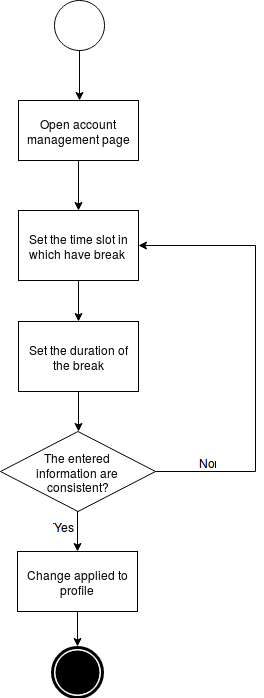
\includegraphics[width=0.5\textwidth]{flows/Scenario8}
	\caption{Activity Diagram : Modify an already compiled schedule for a certain day}
\end{figure}


\newpage
\subsection*{Scenario 9}

Mark has already finish the meeting of the 6pm and he must go to the meeting of 6,30pm, so he opens Travlendar+ application and see the best journey in order to his preferences about means of transport that can permit he to reaches the destination in the way he prefers.
So Mark receive the information about the current journey and all the information about traffic jam, status of public transport service means and strikes that the third part services provide to the application.
\\

\begin{figure}[H]
	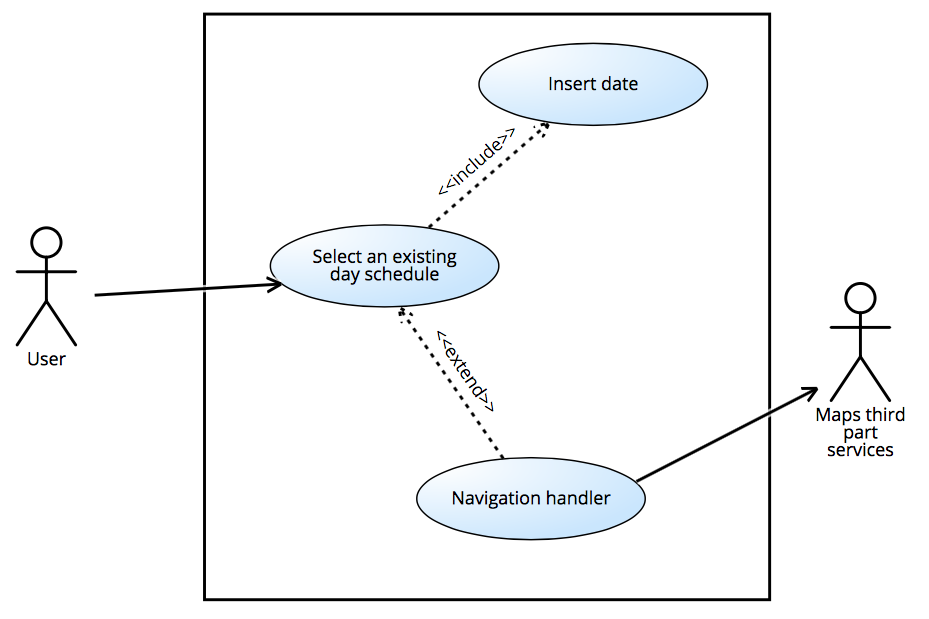
\includegraphics[width=1\textwidth]{usecases/Scenario9}
	\caption{Use Case: Receive information about the current journey}
\end{figure}


\begin{tabular}{|c|p{0.8\textwidth}|}
	\hline
	\parbox[c][6ex]{6ex}{\centering \textbf{Name}} & Receive information about the current journey
	\\
	\hline
	\parbox[c][6ex]{6ex}{\centering \textbf{Actor}} & User, Maps third part services \\
	\hline
	\parbox[c][10ex]{15ex}{\centering \textbf{Entry Condition}} & The user is already logged in to receive the information about the current journey.
	\\
	\hline
	\parbox[c][6ex]{6ex}{\centering \textbf{Goal}} & 9 \\
	\hline
	\parbox[c][10ex]{12ex}{\centering \textbf{Event Flow}} & \begin{itemize}
		\item The user selects from the homepage the event of the current day schedule of which he wants to have the journey
		\item The system shows the event’s information and also the map with the position of the place where the event take place
		\item The user clicks on the map
		\item The system opens the navigation system providing the journey’s information
	\end{itemize}\\
	\hline
	\parbox[c][7ex]{12ex}{\centering \textbf{Exit condition}} & The user reach the destination on time for the next event \\\hline
	\parbox[c][10ex]{13ex}{\centering \textbf{Exceptions}} & The user hasn’t got any events during the current day. If the Location of the device is not available the navigator can provide an error.
	\\ \\ \hline	
	
	
\end{tabular}


\newpage

\begin{figure}[H]
	\centering
	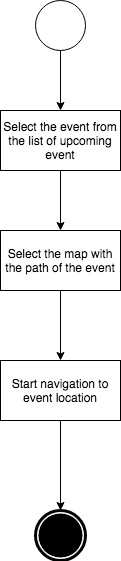
\includegraphics[width=0.3\textwidth]{flows/Scenario9}
	\caption{Activity Diagram : Receive information about the current journey}
\end{figure}
\newpage
\section{Performance Requirements}

As the application will operate in large cities and therefore interacting with many users at the same time, the system must guarantee a certain reliabilty and fault tolerance. In particular, requests to server must be fullfilled within 5 seconds serving up to XXX users (or YYY parallel requests)

\section{Design Constraints}

The system has to memorize and store users' tickets and subscriptions in accordance with the formats provided by the local public transport services. It also has to memorize the users' driving licence with the correct format.

\section{Software System Attributes}

\subsection*{Availability}

The system is requested to have an availability around 98\% corresponding to a maximum downtime of 3.36h per week. In order to achieve this, the server used must be part of a server farm. In this way, even if a single machine ends up being unreachable, the others still work and keep the OS up.

\subsection*{Security}

The system has to guarantee that only users can actually browse and access to all the application's feature, like the creation of a schedule, the purchase of tickets and so on. On the other hand, guests must be able only to check the best route to a certain destination. Moreover, all the users' informations cannot be viewed nor modified by other people. For this purpose the system, before the creation of a new event, requires a login (composed by user and password).\\

It is also fundamental the persistance of such datas, achieved with periodic backups which will be the base of a system recovery. Every exchange of information between server and client must be encrypted in order to avoid leaks of sensitive data.

\subsection*{Portability}

The system must be developed to ease the use of the application on any mobile device. Furthermore, it has to be developed in order to run smoothly on different kinds of tablets or smartphones with several OS like Android, iOS and Windows Phone. The access to the application will be also available from any modern browser on PC.

\subsection*{Maintainability}

The system must be implemented with an architecture that will ease the evolution of the software and its maintainability. For such purpose, the developing will require the use of an Object Oriented Language to partition the code in several classes and make it more readable. It is also required a documentation about the used method's behaviour and guarantee an easy approach to the code in future uses.


\chapter{Formal Analysis using Alloy}

\lstinputlisting{./AlloyDef.als}


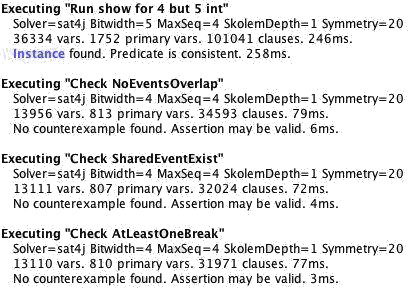
\includegraphics[]{result}

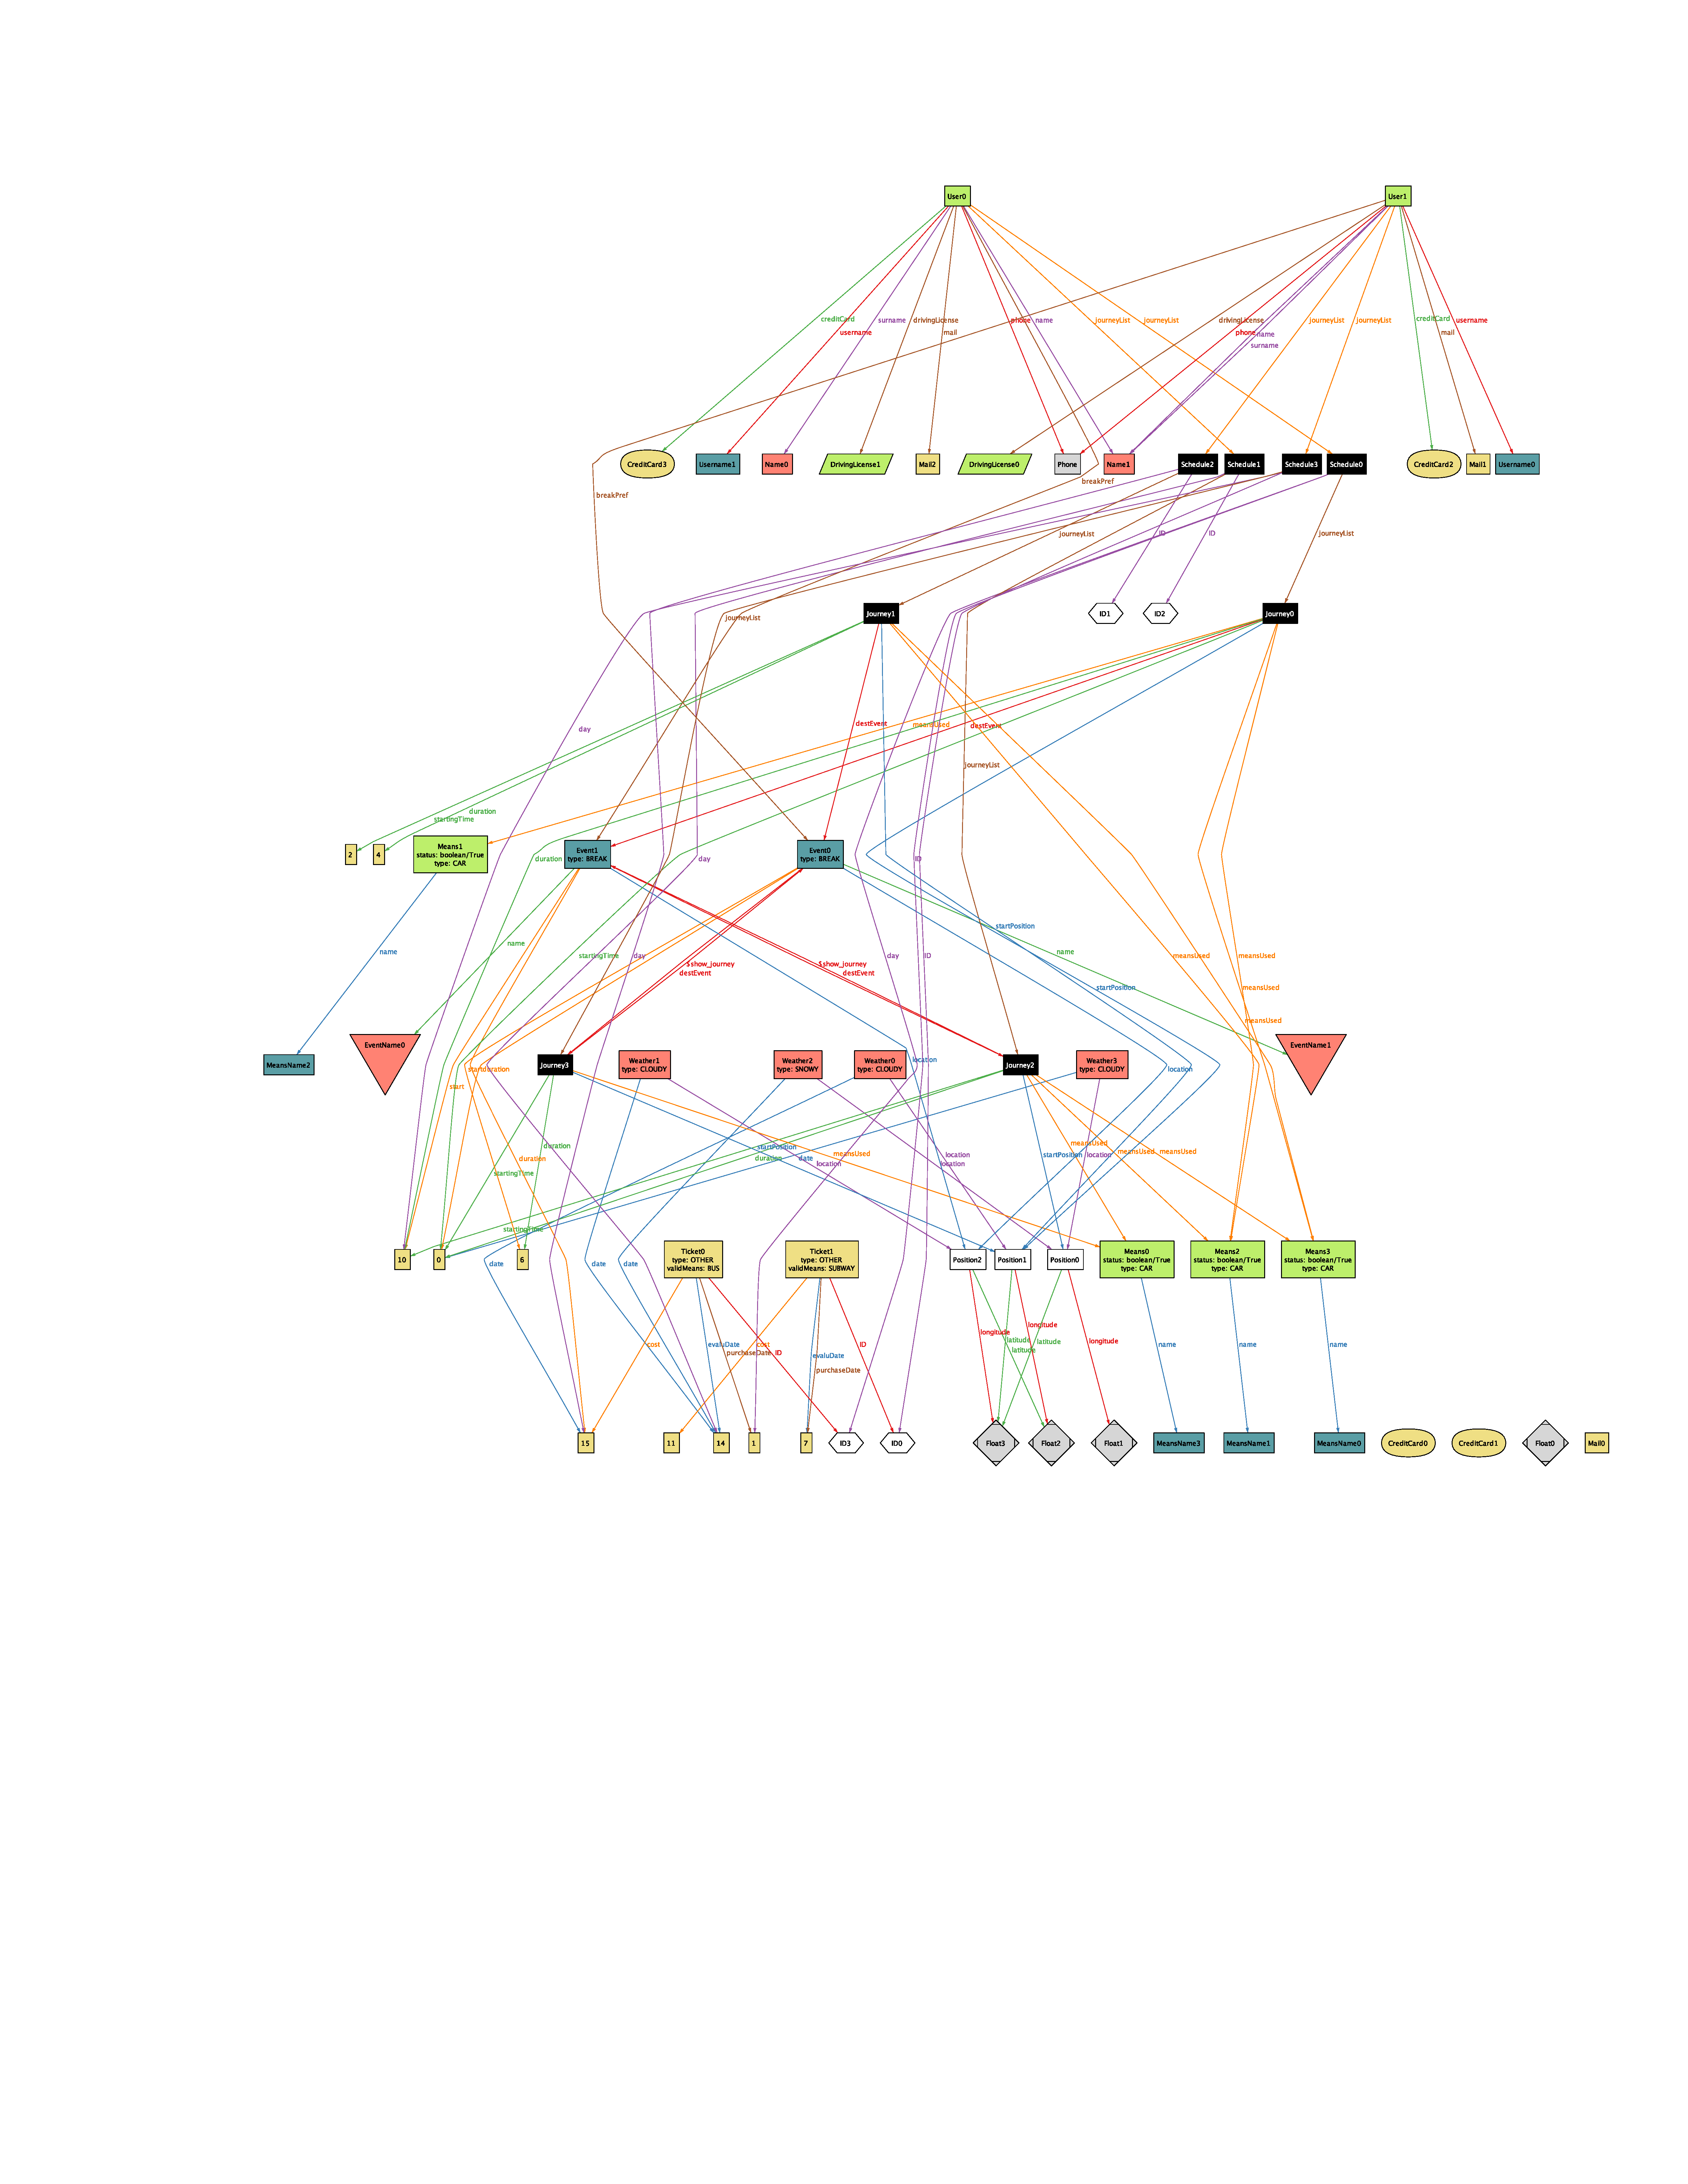
\includepdf[]{AlloyPDFRender.pdf}
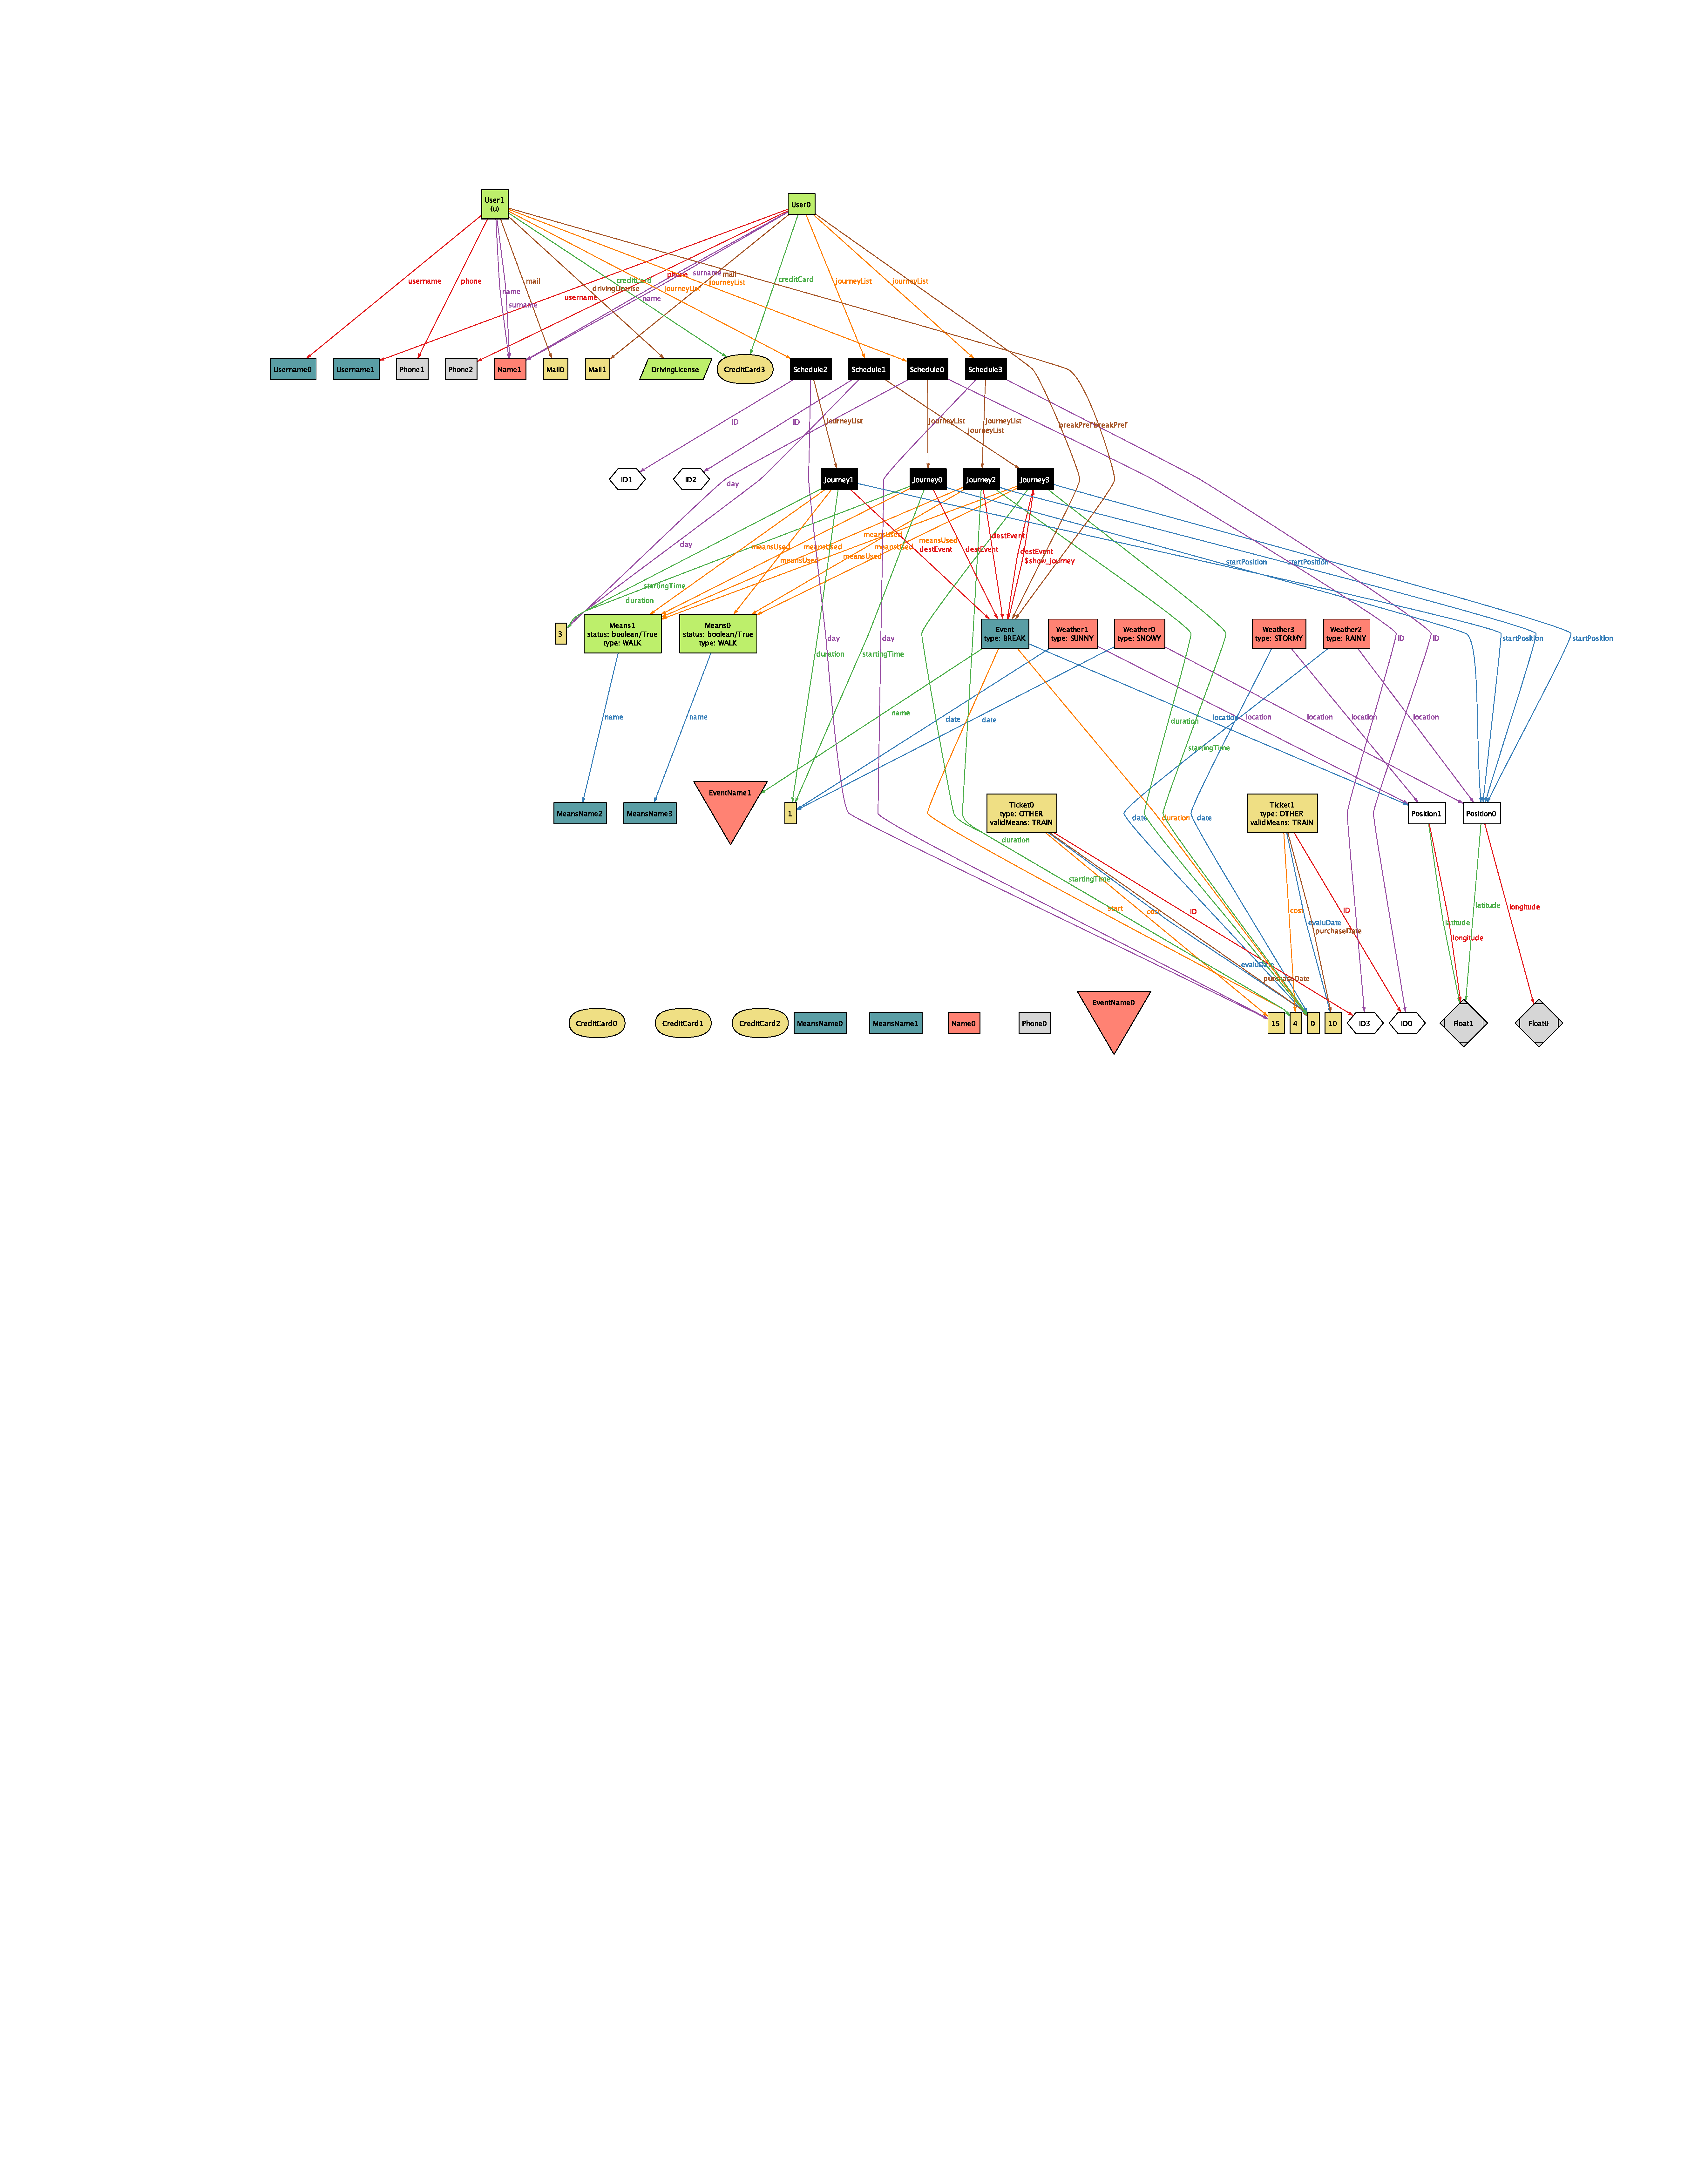
\includepdf[]{PdfAlloy2.pdf}


%\includegraphics[]{AlloyPNGRender}
\chapter{Effort Spent}

While working on the project, we always met to discuss main topics to provide more consistence to the project:\\

\begin{tabular}{|p{0.2\textwidth}|p{0.8\textwidth}|}
	\hline
	\parbox[c][6ex]{6ex}{\centering \textbf{Name}} & \textbf{Effort}
	\\
	\hline
	\parbox[c][8ex]{6ex}{\centering Lukasz Moskwa} & Group 21h and 8h alone\\
	\hline
	\parbox[c][8ex]{6ex}{\centering Marco Mussi} & Group 21h and 8h alone\\
	\hline
	\parbox[c][8ex]{6ex}{\centering Gianluigi Oliva} & Group 21h and 8h alone \\
	\hline
		
	
	
\end{tabular}

\chapter{References}

\begin{itemize}
	\item \textbf{Documentation about availability}:\\ https://en.wikipedia.org/wiki/High\_availability
	\item \textbf{Documentation about alloy}:\\ http://alloy.mit.edu/alloy/
	\item \textbf{Thesis about alloy}:\\ http://computerscience.unicam.it/culmone/?download=\\Tesi\_Claudio\_Vallorani\%28066729\%29.pdf
	\item The orginal Travlendar application: \\
	\textbf{http://score-contest.org/2018/projects/travlendar.php}
	\item The revised document of the assignment:\\
	\textbf{https://goo.gl/9m1ojy}
	\item IEEE Std 830-1998 IEEE Recommended Practice for Software Requirements Specifications. 
	\item IEEE Std 1016tm-2009 Standard for Information Tecnology-System Design-Software Design Descriptions.
\end{itemize}


\end{document}